\documentclass[11pt]{article}
\usepackage[top=1cm, bottom=2cm, left=1cm, right=1cm]{geometry}
\usepackage{ctex}
\usepackage{algorithm}
\usepackage{algorithmicx}
\usepackage{algpseudocode}
\usepackage{amsthm,amsmath,amssymb}
\usepackage[colorlinks=true,linkcolor=blue]{hyperref}
\usepackage{listings}
\usepackage{xcolor,xparse}
\usepackage{realboxes}
\usepackage{graphics}
\usepackage{graphicx}
\usepackage{mathrsfs}
\usepackage{wrapfig}
\usepackage{subfigure}
\usepackage{pifont}
\newcommand{\To}{\textbf{To} }
\definecolor{cmdbg}{rgb}{0.9,0.9,0.9}
\lstset{%
	basicstyle=\ttfamily,
	breaklines = true,
	backgroundcolor=\color{cmdbg},
}
\DeclareDocumentCommand{\ccmd}{v}{% 参数 v 表示工作方法类似于 \verb
    \Colorbox{cmdbg}{\csname lstinline\endcsname!#1!}%
}

\makeatletter
\newenvironment{breakablealgorithm}
  {% \begin{breakablealgorithm}
   \begin{center}
     \refstepcounter{algorithm}% New algorithm
     \hrule height.8pt depth0pt \kern2pt% \@fs@pre for \@fs@ruled
     \renewcommand{\caption}[2][\relax]{% Make a new \caption
       {\raggedright\textbf{\ALG@name~\thealgorithm} ##2\par}%
       \ifx\relax##1\relax % #1 is \relax
         \addcontentsline{loa}{algorithm}{\protect\numberline{\thealgorithm}##2}%
       \else % #1 is not \relax
         \addcontentsline{loa}{algorithm}{\protect\numberline{\thealgorithm}##1}%
       \fi
       \kern2pt\hrule\kern2pt
     }
  }{% \end{breakablealgorithm}
     \kern2pt\hrule\relax% \@fs@post for \@fs@ruled
   \end{center}
  }
\makeatother

\author{谢昀城 22307110070}
\title{计算物理作业3}

\begin{document}
\maketitle


\section{题目1:计算LU分解的复杂度}
\subsection{题目描述}
Prove that the time complexity of the LU compositionde algorithm is $O(N^3)$

\subsection{证明}
对于将矩阵$A$分解为上三角矩阵$U$和下三角矩阵$L$,即:
$$
\begin{pmatrix}
  a_{11} & a_{12} & \cdots & a_{1n} \\
  a_{21} & a_{22} & \cdots & a_{2n} \\
  \vdots & \vdots & \ddots & \vdots \\
  a_{n1} & a_{n2} & \cdots & a_{nn}
  \end{pmatrix}=\begin{pmatrix}
    1 & 0 & \cdots & 0 \\
    l_{21} & 1 & \cdots & 0 \\
    \vdots & \vdots & \ddots & \vdots \\
    l_{n1} & l_{n2} & \cdots & 1
    \end{pmatrix}
    \begin{pmatrix}
      u_{11} & u_{12} & \cdots & u_{1n} \\
      0 & u_{22} & \cdots & u_{2n} \\
      \vdots & \vdots & \ddots & \vdots \\
      0 & 0 & \cdots & u_{nn}
      \end{pmatrix}
$$
同时有$A^{T}=U^{T}L^{T}$,因此我们可以交替计算$U$的第$i$行和$L$的第$i$列,计算过程如下:


\begin{breakablealgorithm}
  \caption{LU Decomposition}
  \begin{algorithmic}

\For{$i \gets 1$ \To $N$}
\For{$j \gets i$ \To $N$}

$u_{ij} \gets a_{ij}-\sum_{k=1}^{i-1} l_{i,k} u_{k,j}$ \Comment{total of $i$ computations}

\EndFor  \Comment{total of $i\times (N-i+1) $ computations}

\For {$j \gets i+1$ \To $N$}

    $l_{ji} \gets a_{ji}-{1 \over u_{kk}}\sum_{k=1}^{i-1} l_{i,k} u_{k,j}$ \Comment{total of $i+1$ computations}

\EndFor \Comment{total of $(i+1) \times (N-i)$ computations}
\EndFor

  \end{algorithmic}
  \end{breakablealgorithm}
因此,LU分解复杂度为:
$$\sum_{i=1}^{N} i(N-i+1)+(i+1)(N-i)=N+\sum_{i=1}^{N} 2Ni-4\sum_{i=1}^{N} i^2=N^2(N+1)-{2 \over 3}N(N+1)(N+2)+N \approx O(N^3)$$



\section{题目 2:}
\subsection{题目描述}
.用Gaussian elimination algorithm和partial-pivoting scheme求解方程组:
$$
2x_1+3x_2+5x_3=5
$$

$$
3x_1+4x_2+8x_3=6
$$

$$
x_1+3x_2+3x_3=5
$$
\subsection{程序描述}
在本程序中,我们使用最大主元的高斯消元法来求解方程组。其中partial\_pivoting\_scheme函数用于将大于最大主元行交换到i位置。guaussian\_elimination函数用于进行高斯消元法求解方程组,返回增广矩阵的消元结果,解和求解情况flag。正常求解,flag=0;无解:x=nan,flag=2;无穷解,flag=1,程序将返回其中的一组解。

程序源文件为gaussian\_elimination.py,将输入方程系数以逗号分隔写于MatrixIn.txt文件中并置于统一文件夹下,在终端进入当前目录,使用命令python -u gaussian\_elimination.py运行本程序。运行时请保证Python第三方库Numpy已安装。程序开发环境为Python3.12.3,可在Python3.8以上版本中运行。

\subsection{伪代码}
\begin{breakablealgorithm}
  \caption{PartialPivotingScheme}
  \begin{algorithmic}
    \Function{PartialPivotingScheme}{$M, i$}
      \State \textbf{INPUT:} $M$ (2D array), $i$ (integer)
      \State \textbf{OUTPUT:} $reM$ (2D array)
      \State $reM \gets M$ 
      \State $maxIndex \gets i + ArgMax(|(M[i:, i]|)$
      \If {$i \neq maxIndex$}
        \State $reM[maxIndex, :] \gets M[i, :]$\Comment{Swap the rows}
        \State $reM[i, :] \gets M[maxIndex, :]$
      \EndIf
      \State \Return $reM$
    \EndFunction
  \end{algorithmic}
  \end{breakablealgorithm}
  
  \begin{breakablealgorithm}
    \caption{GaussianElimination}
    \begin{algorithmic}
      \Function{GaussianElimination}{$M$}
        \State \textbf{INPUT:} $M$ (2D array)
        \State \textbf{OUTPUT:} $Me$ (2D array), $x$ (1D array), $flag$ (integer)
        \State $Me \gets M$ 
        \State $flag \gets 0$
        \State $row \gets$ size($Me$, 0) \Comment{Forward elimination}
        \For{$i \gets 0$ \To $row-1$}
          \State $Me \gets$ PartialPivotingScheme($Me, i$)
          \For{$j \gets i+1$ \To $row-1$}
            \State $Me[j, :] \gets Me[j, :] - Me[i, :] * Me[j, i] / Me[i, i]$
          \EndFor
        \EndFor \Comment{Backward substitution}
        \State $x \gets$ zeros($row$)
        \For{$i \gets row-1$ \To $0$ \textbf{step} $-1$}
          \For{$j \gets row-1$ \To $i+1$ \textbf{step} $-1$}
            \State $x[i] \gets x[i] - Me[i, j] * x[j]$
          \EndFor
          \State $x[i] \gets x[i] + Me[i, -1]$
          \If {$Me[i, i] = 0$ and $x[i] \neq 0$}
            \State $flag \gets 2$
            \State \Return $Me$, $nan$, $flag$
          \EndIf
          \If {$Me[i, i] = 0$ and $x[i] = 0$}
            \State $x[i] \gets 1$
            \State $flag \gets 1$
            \State \textbf{continue}
          \EndIf
          \State $x[i] \gets x[i] / Me[i, i]$
        \EndFor
        \State \Return $Me$, $x$, $flag$
      \EndFunction
    \end{algorithmic}
    \end{breakablealgorithm}
    
  \subsection{输入输出实例}
  对于本程序,运行后读取MatrixIn.txt文件中的系数矩阵,输出增广矩阵的消元结果,解和求解情况。程序运行截图如图\ref{fig:1}所示。程序得到方程组的解为$x_1=2,x_2=2,x_3=-1$
  此外,图\ref{fig:2}\ref{fig:3}展示了无解和无穷解的程序输出情况。

  \begin{figure}[ht]
    \centering
    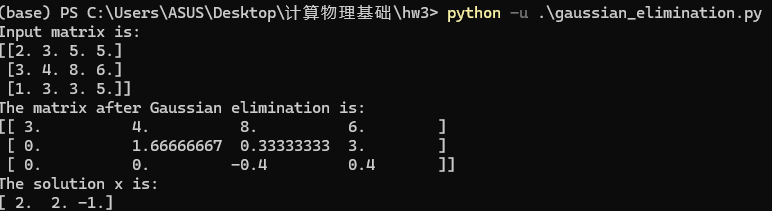
\includegraphics[width=0.6\linewidth]{photo/fig1.png}
    \caption{题目2程序运行截图}
    \label{fig:1}
  \end{figure}
  \begin{figure}[ht]
    \centering
    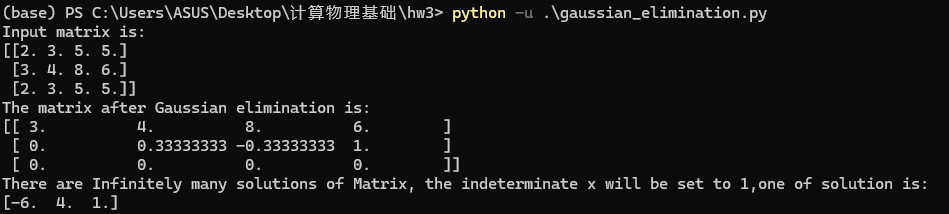
\includegraphics[width=0.6\linewidth]{photo/fig2.png}
    \caption{题目2程序运行截图:无穷解情况}
    \label{fig:2}
  \end{figure}
  \begin{figure}[ht]
    \centering
    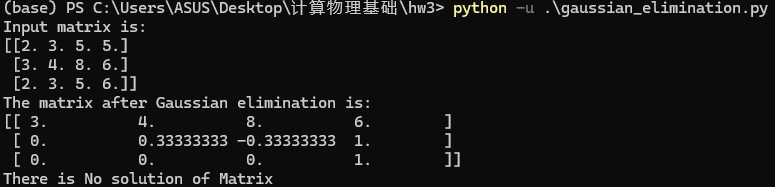
\includegraphics[width=0.6\linewidth]{photo/fig3.png}
    \caption{题目2程序运行截图:无解情况}
    \label{fig:3}
  \end{figure}

  \section{题目3}
  \subsection{题目描述}
  Solve the 1D Schrodinger equation with the potential (i)$V(x)=x^2 $(ii)
  $V(x)=x^4-x^2$ 
  with the variational approach using a Gaussian basis (either fixed widths or fixed centers). Consider the three lowest energy eigenstates.  The Gaussian basis functions are defined as: $\phi_i(x)=({v_i\over \pi}^(1/2)e^(-v_i(x-s_i)^2))$his function has two variational parameters:
$v_i$, the width of the Gaussian, and $s_i$
  , the center of the Gaussian. For simplicity, we only vary one of these parameters at a time and do calculations with either fixed widths or fixed centers. 


\subsection{程序描述}
在本程序中,我们通过将波函数在高斯基上展开,并求解关于系数的广义本征值问题$HC=ESC$,以得到$V(x)=x^2$和$V(x)=x^4-x^2$的$n=1,2,3$时的能量和波函数。

其中:
$$
H_{ij} = \langle \phi_i | \hat{H} | \phi_j \rangle, \quad S_{ij} = \langle \phi_i | \phi_j \rangle,\Psi(x)=\sum C_i \phi_i(x)  
$$

由于$V(x)$关于$x=0$对称,波函数将存在奇宇称和偶宇称两种情况,而高斯基关于$s_i$对称,因此我们固定$v_i$,变化$s_i$将会得到更好的效果。

因此,本程序中我们固定$v_i=1$,在$(-20,20)$范围内,均匀选取100组$s_i$展开波函数$\Psi$,
并且使用scipy库中的eigh函数求解广义本征值问题,得到特征值值和归一化特征向量,最终得到最低的三个能级能量和波函数。

为方便我们选取单位为$\bar{h}=1,m=1$,
因此$\hat{H}=-{1\over 2}{d^2\over dx^2}+V(x)$
可以得到:
$$
S_{Si,Sj}=\frac{e^{-\frac{1}{2} (S_i - S_j)^2}}{\sqrt{2 \pi}}
$$
对$V(x)=x^2$:
$$
H_{S_i,S_j}=\frac{e^{-\frac{1}{2} (S_i - S_j)^2} \left( -3 + S_i^2 - 6 S_i S_j + S_j^2 \right)}{4 \sqrt{2 \pi}}
$$
对$V(x)=x^4-x^2$:
$$
H_{S_i,S_j}=\frac{e^{-\frac{1}{2} (S_i - S_j)^2} \left( 7 + S_i^4 + 4 S_i^3 S_j - 6 S_j^2 + S_j^4 + 6 S_i^2 (-1 + S_j^2) + 4 S_i S_j (5 + S_j^2) \right)}{16 \sqrt{2 \pi}}
$$

本程序源文件为SchrodingerEq.py,在终端进入当前目录,使用命令python -u SchrodingerEq.py运行本程序。运行时请保证Python第三方库Numpy,Matplotlib,scipy已安装。程序开发环境为Python3.12.3,可在Python3.8以上版本中运行。

\subsection{伪代码}
\subsubsection{Trapezoidal integrate 伪代码:}

\begin{breakablealgorithm}
  \caption{SolveSchrodingerEq}
  \begin{algorithmic}
  \For{$i \gets 0$ \To $N$}
    \For{$j \gets 0$ \To $N$}
      \State $H_{ij}\gets \langle \phi_i | \hat{H} | \phi_j \rangle$
      \State $S_{ij} \gets  \langle \phi_i | \phi_j \rangle$
    \EndFor
  \EndFor
  \State $E, C \gets eigh(H, S)$
  \For{$i \gets 0$ \To $3$}

    $Energy_i\gets E[i]$

    $\Psi_i(x)=\gets \sum C_i \phi_i(x)$
  \EndFor
  \end{algorithmic}
  \end{breakablealgorithm}
  
  
  \subsection{输入输出实例}
  对于本程序,运行后会生成两种势能下的归一化波函数和势能图\ref{fig:4}和\ref{fig:5},分别为"wavefunction of V=x\^2.png"和"wavefunction of V=x\^4-x\^2.png",于当前目录下,并输出两种势能下的最低三个能级能量。程序运行截图如图\ref{fig:6}所示。得到能量为($\bar{h}=1,m=1$):
  $$
  V(x)=x^2: E_0=0.70710678,E_1=2.12132034,E_2=3.53553391
  $$
  $$
  V(x)=x^4-x^2: E_0=0.33796154,E_1=1.61273703,E_2=3.66191064
  $$

 
  \begin{figure}[ht]
    \centering
    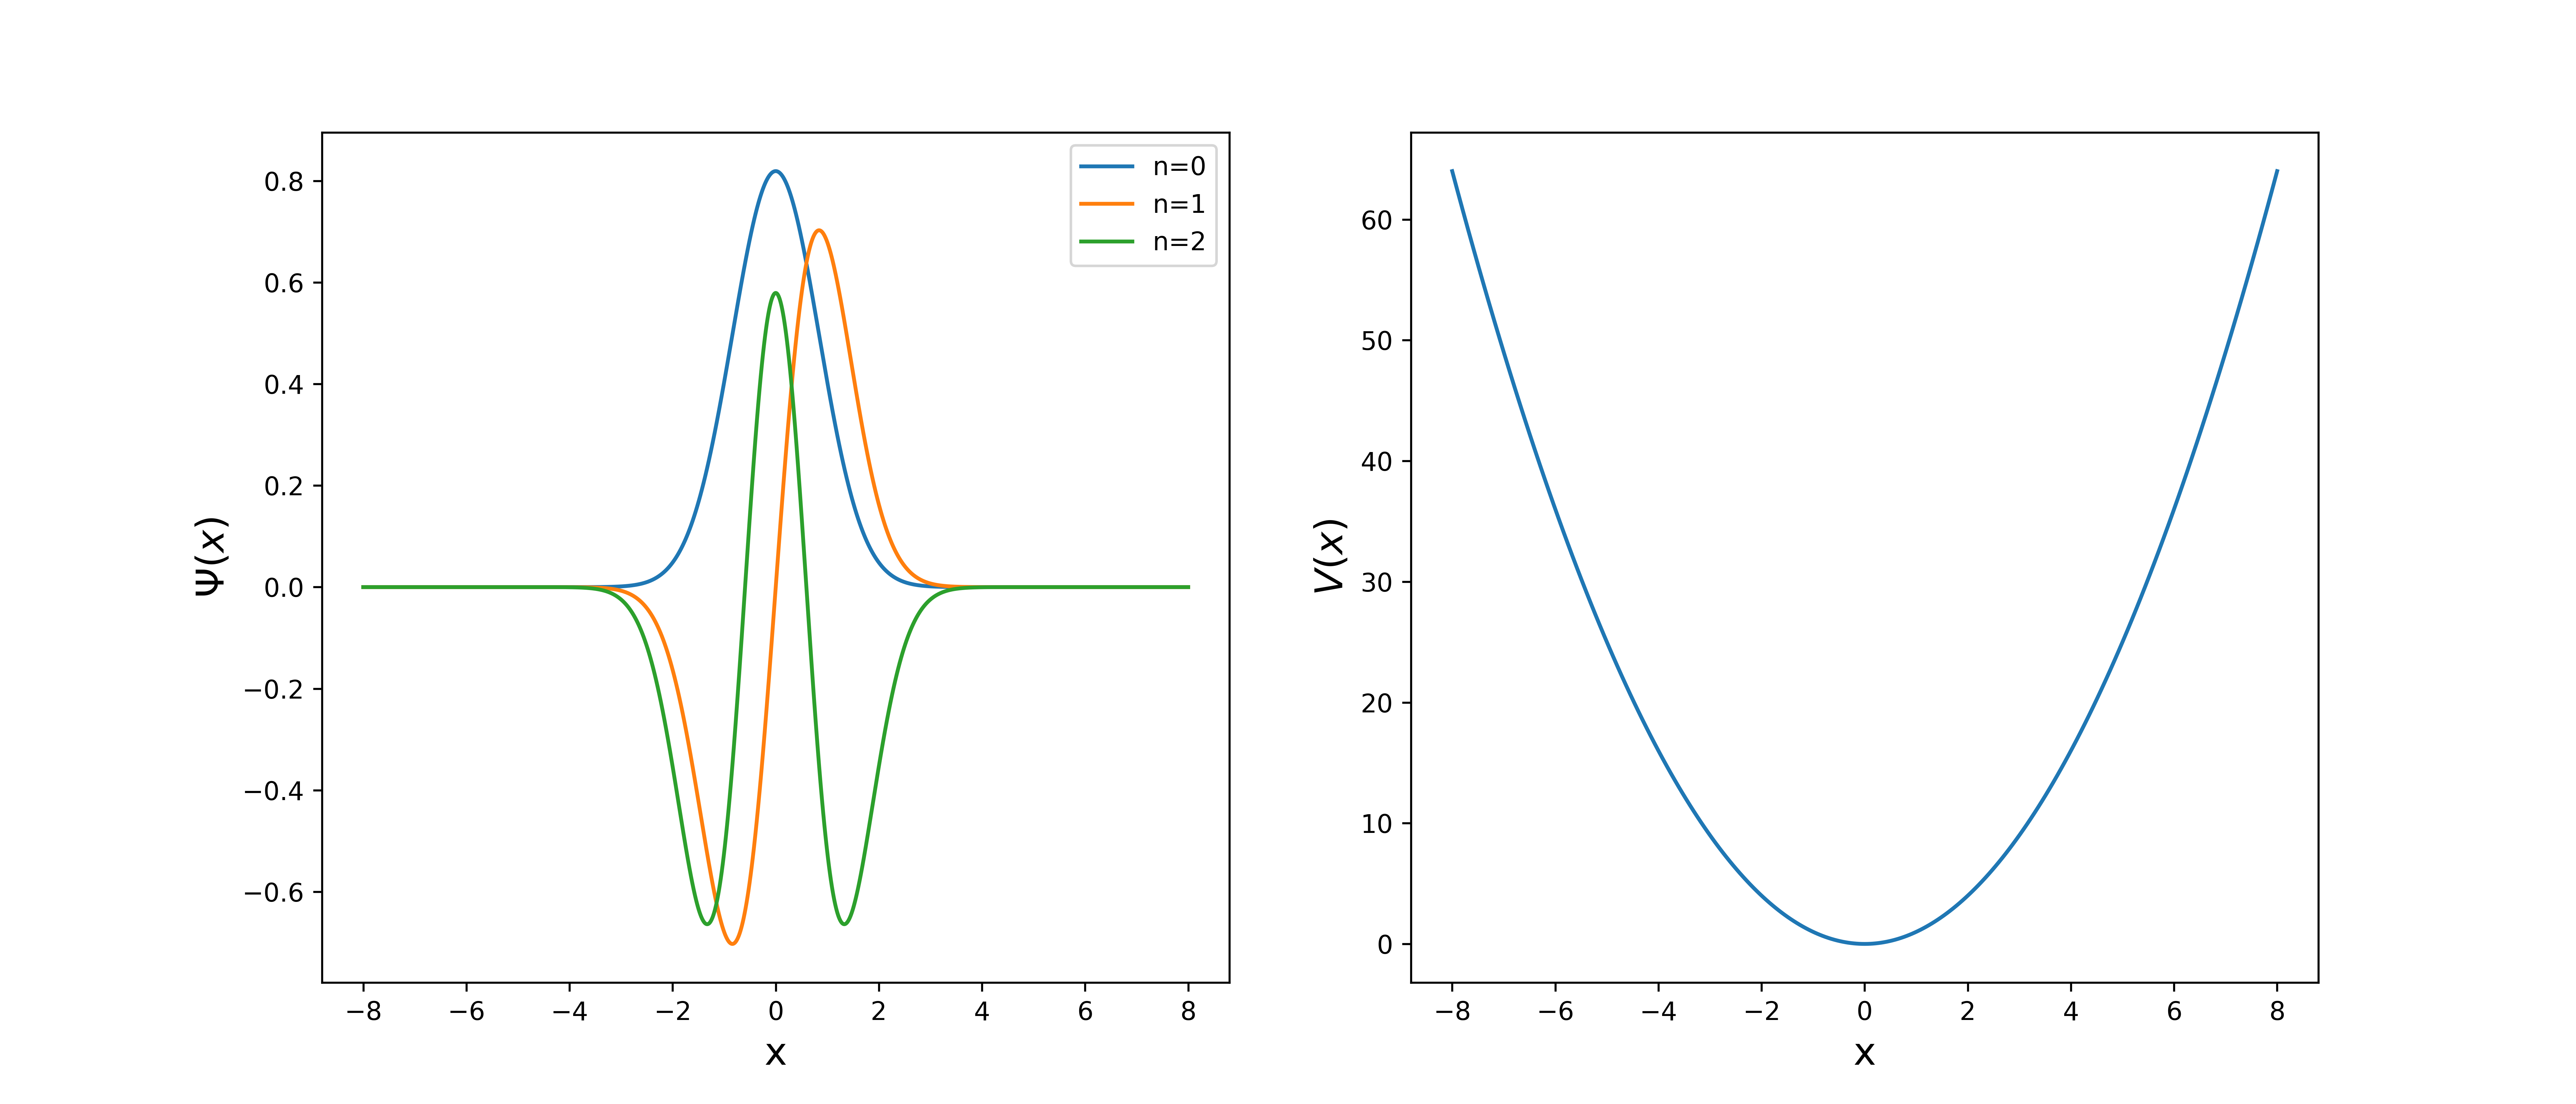
\includegraphics[width=0.8\linewidth]{photo/wavefunction of V=x^2.png}
    \caption{$V(x)=x^2$时的归一化波函数和势能}
    \label{fig:4}
  \end{figure}

  \begin{figure}[ht]
    \centering
    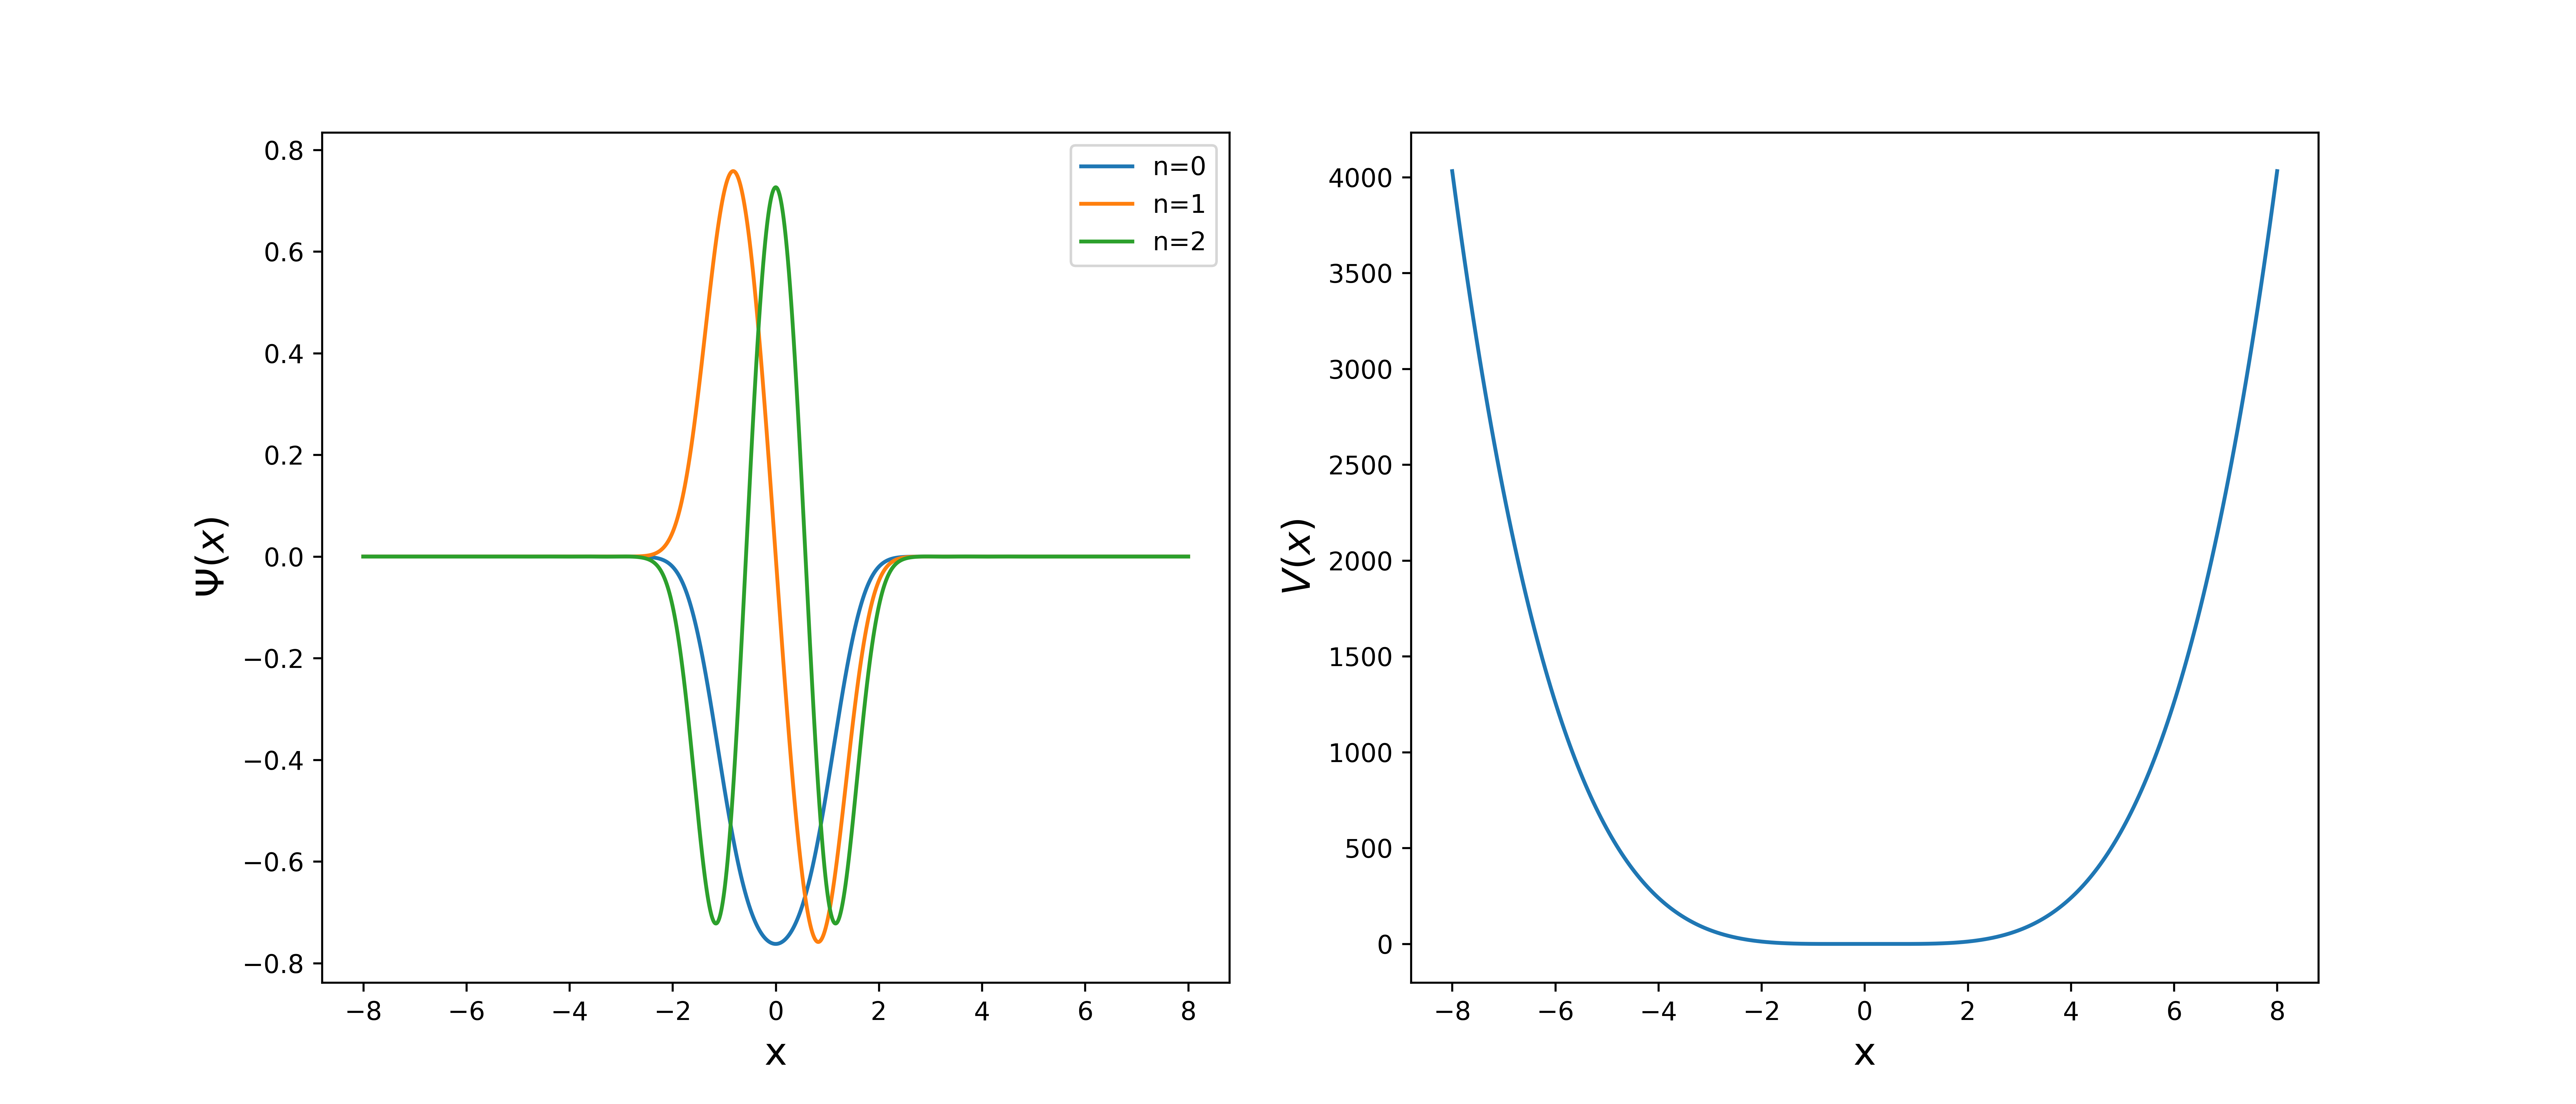
\includegraphics[width=0.8\linewidth]{photo/wavefunction of V=x^4-x^2.png}
    \caption{$V(x)=x^4-x^2$时的归一化波函数和势能}
    \label{fig:5}
  \end{figure}

  \begin{figure}
    \centering
    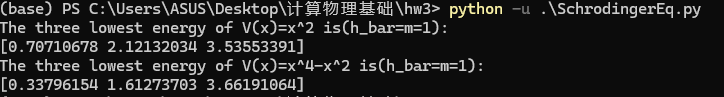
\includegraphics[width=0.6\linewidth]{photo/fig4.png}
    \caption{题目3程序运行截图}
    \label{fig:6}
  \end{figure}

  

\end{document}


